\section{Time Series Analysis}
We decided to do task 4.1 as last part of the project which expected us to find groups of similar cities given their temperature trends. Figure \ref{fig:timeseries_dataset} shows the initial dataset and the modified one, built with the pivot method from pandas, on which we worked on during our analysis. The resulting dataframe now has the cities as indexes and the temperature records as values, so it made our task easier.
\begin{figure}[H]
    \centering
    \subfloat[Initial dataset]{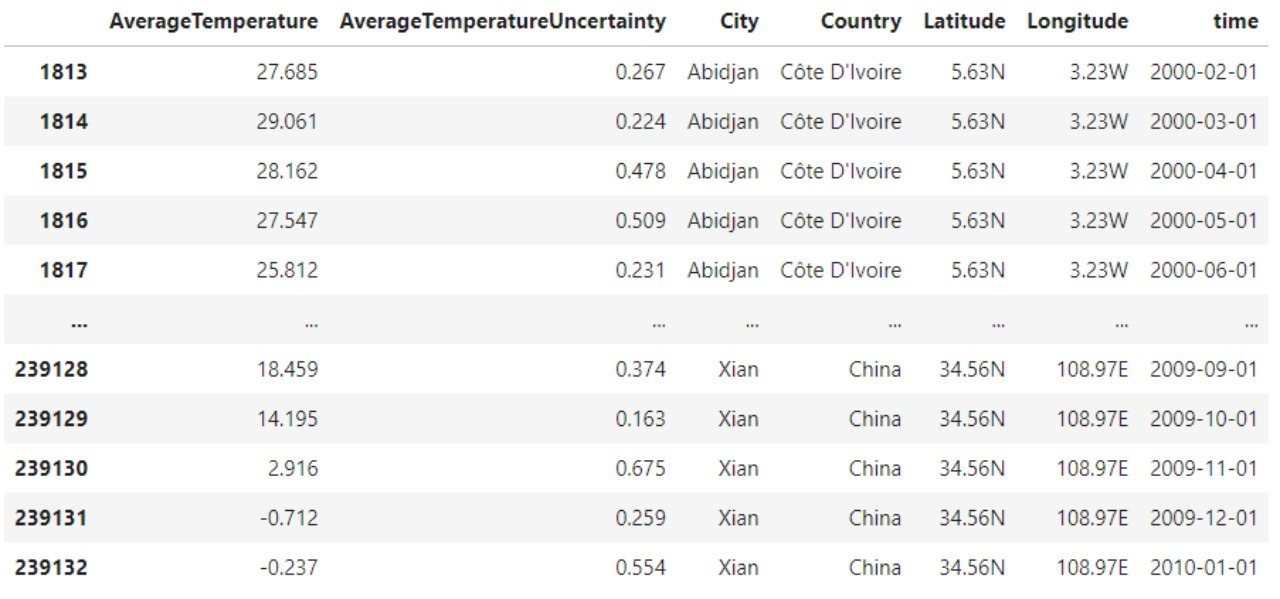
\includegraphics[width=0.45\linewidth]{images/time_series_analysis/timeseries_dataset.jpg}}
    \subfloat[The organized dataset]{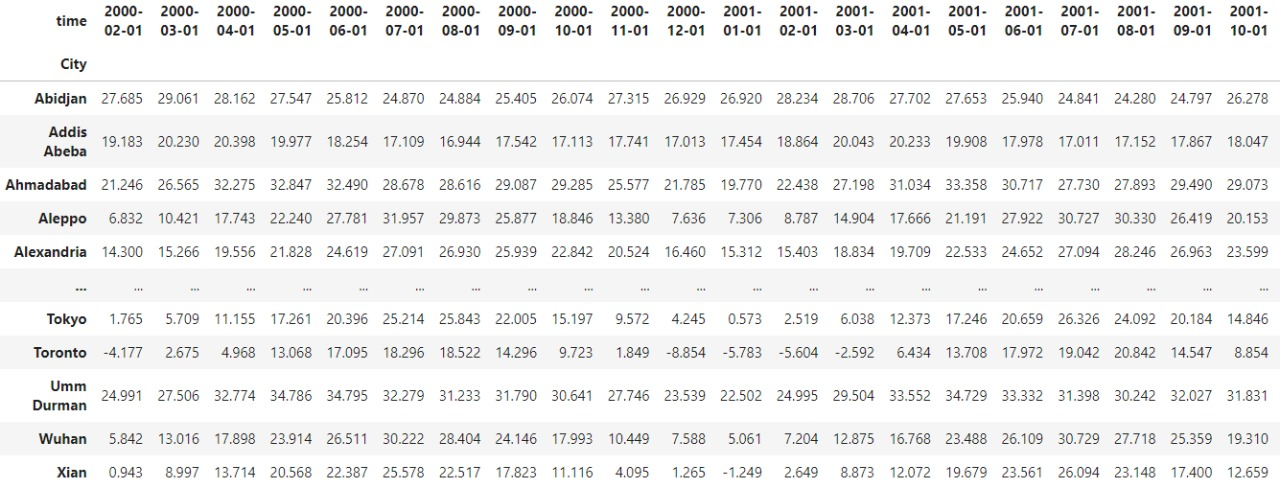
\includegraphics[width=0.55\linewidth]{images/time_series_analysis/timeseries_dataset_modified.jpg}}
    \caption{Time series dataset before and after using the pivot method from pandas.}
    \label{fig:timeseries_dataset}
\end{figure}
Then we used the k-means clustering from the tslearn package to choose the best values of k (the number of clusters) based, as seen during the clustering task, on the SSE, silhouette and Davies-Bouldin scores. Afterwards, we took the best k value and we use it to do the definitive clustering on the cities dataframe.
\begin{figure}[H]
    \centering
    \subfloat[Scores]{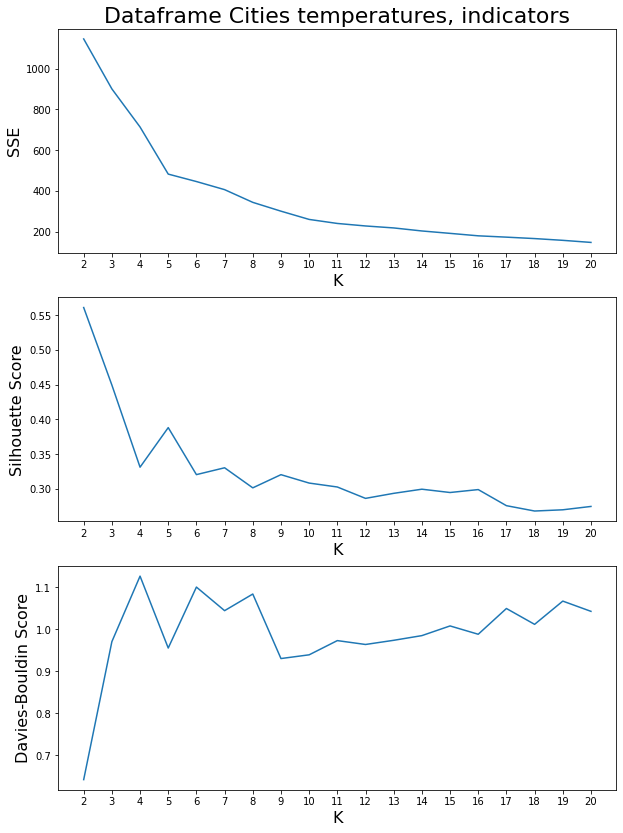
\includegraphics[width=0.38\linewidth]{images/time_series_analysis/timeseries_k.png}}
    \subfloat[The plot with k=5]{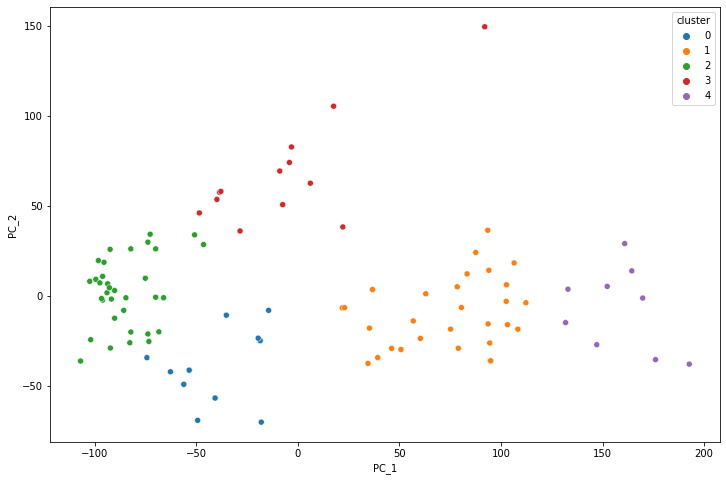
\includegraphics[width=0.62\linewidth]{images/time_series_analysis/timeseries_plot_cluster.png}}
    \caption{Scores for each value of k and clustering with the best k value.}
    \label{fig:timeseries_clusters}
\end{figure}
As figure \ref{fig:timeseries_clusters} on the left shows, by using the elbow rule and by looking at the other two values we took 5 as the best value for k on which we did the final clustering analysis whose plot is still shown on \ref{fig:timeseries_clusters}.
\vspace{3mm}

The cities are, therefore, separated in five different cluster in accordance to their temperature trend:
\begin{itemize}
    \item Cluster 0, warm winter and very hot summer.
    \item Cluster 1, cold winter and hot summer.
    \item Cluster 2, very hot winter and very hot summer.
    \item Cluster 3, warm winter and mild summer.
    \item Cluster 4, very cold winter and mild summer
\end{itemize}
We then plotted those temperature trends and also we plotted the cities on a map according to the cluster they belong to.
\begin{figure}[H]
    \centering
    \subfloat[Cluster trends]{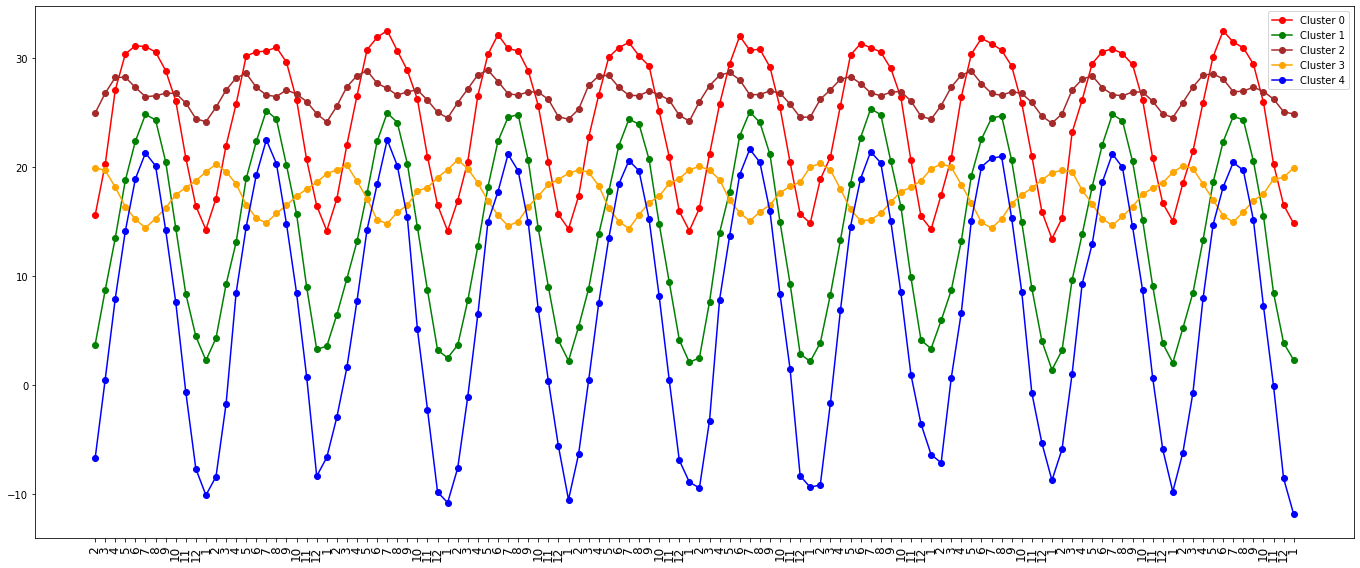
\includegraphics[width=0.41\linewidth]{images/time_series_analysis/timeseries_plot.png}}
    \subfloat[Cluster map]{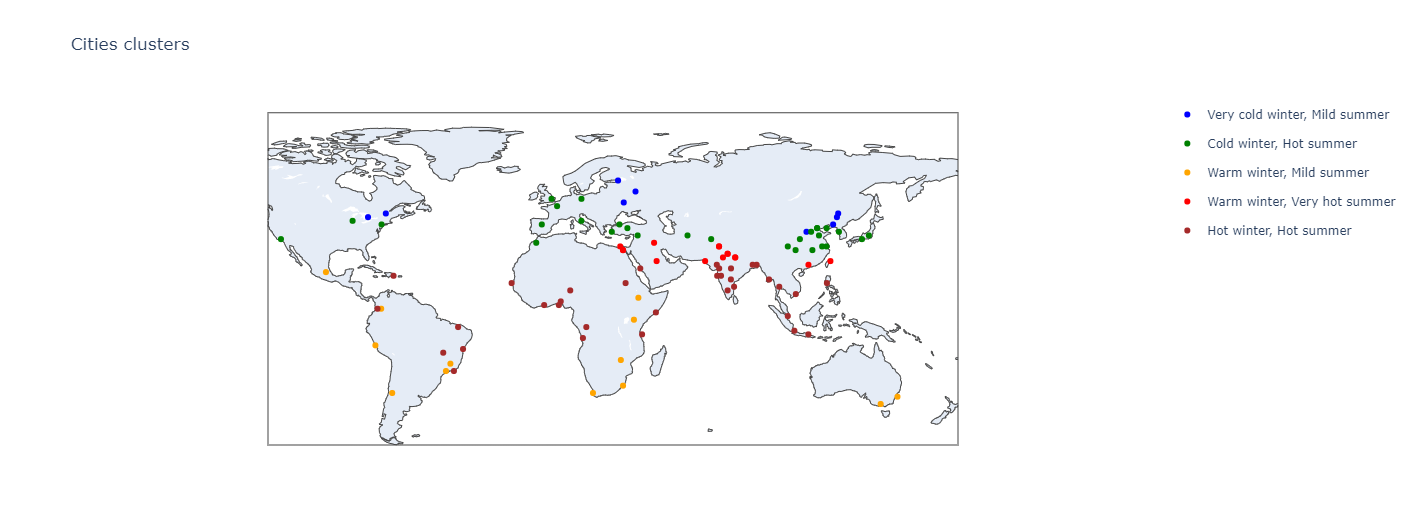
\includegraphics[width=0.59\linewidth]{images/time_series_analysis/timeseries_map.png}}
    \caption{Temperature trends for each cluster and the map with the cities plotted with respect to the cluster they belong to.}
    \label{fig:timeseries_plot_map}
\end{figure}
The map in figure \ref{fig:timeseries_plot_map} shows that cities in similar clusters are somewhat at the same latitude (which is something that we expected), there could have benn some outliers due to the altitude but, luckily, this wasn't the case.